\documentclass[12pt,a4paper,titlepage]{scrartcl}

\usepackage{comment}
\usepackage[main=ngerman,english]{babel}
\usepackage[utf8]{inputenc}
\usepackage[T1]{fontenc}
\usepackage{lmodern}
\usepackage{geometry}
\geometry{left=2.5cm,right=2.5cm,top=2.5cm,bottom=3cm,head=29pt,foot=25pt}
\setlength{\footheight}{25pt}
\usepackage{microtype}
\usepackage{amsmath,amssymb,mathtools}
\numberwithin{equation}{section}
\numberwithin{table}{section}
\numberwithin{figure}{section}
\usepackage{siunitx}
\sisetup{locale=DE, separate-uncertainty=true, per-mode=fraction}
\usepackage{booktabs}
\usepackage{multirow}
\usepackage{graphicx}
\usepackage{float}
\usepackage{caption}
\usepackage{subcaption}
\usepackage[automark]{scrlayer-scrpage}
\usepackage[most]{tcolorbox}
\usepackage{hyperref}
\usepackage{pdfpages}
\usepackage{csvsimple-l3}
\usepackage{longtable}
\usepackage{graphicx}

\input{../../jupyterpackages.tex}


\newcommand{\pdfabbildung}[2]{%
    \refstepcounter{figure}%
    \addcontentsline{lof}{figure}{\protect\numberline{\thefigure}#1}%
    \label{#2}%
}

\newcommand{\pdftabelle}[2]{%
    \refstepcounter{table}%
    \addcontentsline{lot}{table}{\protect\numberline{\thetable}#1}%
    \label{#2}%
}


\hypersetup{colorlinks=true, linkcolor=blue!60!black, urlcolor=blue!60!black, citecolor=blue!60!black}

\clearpairofpagestyles

\chead{%
    \versuch\hfill\autor\\
    \rule{\textwidth}{0.2pt}%
}
\cfoot{%
    \rule{\textwidth}{0.2pt}\\[-0.5ex]
    \pagemark\ 
}
\addtokomafont{pagefoot}{\small}
\setlength{\parindent}{0pt}

\newtcolorbox{resultbox}[1][]{ 
    enhanced,
    colback=black!4!white,
    colframe=black!65!black,
    boxrule=0.8pt,
    arc=0.0mm,
    title=#1,
    fonttitle=\bfseries,
    %drop shadow
}


\newcommand{\versuch}{Versuch 26}
\newcommand{\titel}{Schallgeschwindigkeit}
\newcommand{\praktikum}{Physikalisches Anfängerpraktikum 1}
\newcommand{\autor}{Jonathan Gießen}
\newcommand{\gruppe}{Gruppe 8}
\newcommand{\datum}{7. September 2026}
\newcommand{\betreuer}{Pia Franz}

\begin{document}

\pagestyle{scrheadings}

\begin{titlepage}



    \centering
    \vspace*{4cm}
    {\large Universität Heidelberg\par}
    {\small Fakultät für Physik und Astronomie\par}
    {\Large \praktikum\par}
    \vspace{0.8cm}
    {\LARGE \bfseries \versuch\ -- \titel\par}
    \vspace{1.5cm}

    \begin{tabular}{ll}
        \textbf{Autor:} & \autor\\
        \textbf{Gruppe:} & \gruppe\\
        \textbf{Betreuer:} & \betreuer\\
        \textbf{Versuchsdatum:} & \datum\\
    \end{tabular}

    \vfill
    \hrulefill\
\end{titlepage}

\tableofcontents

\bigskip
\begin{tcolorbox}[colback=gray!5,colframe=gray!60,boxrule=0.8pt,arc=0.01mm,title=KI-Hinweis]
    Für die sprachliche Formulierung dieses Protokolls wurde in Teilen KI-gestützte Textgenerierung verwendet. 
\end{tcolorbox}


\clearpage
\section{Einleitung}
Ziel des vorliegenden Versuchs aus dem Physikalischen Anfängerpraktikum ist die experimentelle Bestimmung der Schallgeschwindigkeit in den Gasen Luft und Kohlenstoffdioxid ($CO_2$). Die Ausbreitungsgeschwindigkeit von Schall in Gasen hängt maßgeblich von deren thermodynamischen Eigenschaften ab, wie etwa dem Adiabatenkoeffizienten ($\kappa$), der Molmasse ($M$) sowie der Umgebungstemperatur ($T$). Um diese Zusammenhänge zu untersuchen, werden im Rahmen dieses Versuchs zwei unterschiedliche experimentelle Methoden angewandt.

Im ersten Versuchsteil wird die Schallgeschwindigkeit mithilfe von stehenden Wellen in einem sogenannten Quincke'schen Rohr bestimmt. Eine von einem Lautsprecher erzeugte Schallwelle trifft in dem Rohr auf eine verstellbare Wasseroberfläche, wird an dieser reflektiert und interferiert mit der einfallenden Welle. Durch das Heben und Senken des Wasserspiegels wird die effektive Länge der Luftsäule variiert, wodurch Resonanzfälle eingestellt werden können. Im Resonanzfall befindet sich am Ort des Schallgebers ein Wellenbauch und am Wasser-Reflektor ein Wellenknoten. Um das empfangene Mikrofonsignal von Rauschen und Störgeräuschen zu befreien und die Lautstärkemaxima präzise ermitteln zu können, kommt ein Lock-In-Verstärker zum Einsatz. Aus den Höhendifferenzen zwischen den Resonanzmaxima lässt sich die Wellenlänge und somit die Schallgeschwindigkeit für Luft und $CO_2$ berechnen. Um die Messungen vergleichbar zu machen, werden die bei Raumtemperatur ermittelten Werte anschließend theoretisch auf Normalbedingungen ($0^{\circ}\text{C}$) umgerechnet.

Im zweiten Versuchsteil erfolgt die Bestimmung der Schallgeschwindigkeit (nur für Luft) durch die Laufzeitmessung einer fortschreitenden Schallwelle. Hierbei wird mit einem Zweikanal-Oszilloskop die Phasenverschiebung zwischen dem Sendesignal eines Sinusgenerators und dem von einem verschiebbaren Mikrofon empfangenen Signal gemessen. Durch die Untersuchung der Weglängenänderung zwischen Mikrofon und Lautsprecher, bei der sich die Phase auf dem Oszilloskop um genau eine Wellenlänge (bzw. eine Periode) verschiebt, kann die Ausbreitungsgeschwindigkeit des Schalls ermittelt werden.

Beide Verfahren erlauben abschließend einen direkten Vergleich der experimentell gewonnenen Werte mit den theoretisch erwarteten Schallgeschwindigkeiten.

\section{Grundlagen und Theorie}
\subsection{Physikalische Formeln}
Beim Schall handelt es sich um eine mechanische Welle, die sich in einem Medium ausbreitet. Die Geschwindigkeit, mit der sich Schallwellen fortbewegen, hängt von den Eigenschaften des Mediums ab, insbesondere von dessen Dichte und Elastizität. In Gasen, wie Luft, kann die Schallgeschwindigkeit durch die Temperatur beeinflusst werden.

Grundlegend kann die Schallgeschwindigkeit $c$ in einem idealen Gas durch die folgende Formel beschrieben werden:
\begin{equation}
    c = \sqrt{\frac{\kappa \cdot R \cdot T}{M}}\label{eq:schallgeschwindigkeit aus Theorie}
\end{equation}
wobei $\kappa$ der Adiabatenkoeffizient, $R$ die universelle Gaskonstante, $T$ die absolute Temperatur und $M$ die molare Masse des Gases ist.
Für Wellen gilt die Beziehung zwischen Frequenz $f$, Wellenlänge $\lambda$ und Schallgeschwindigkeit $c$:
\begin{equation}
    c = f \cdot \lambda \label{eq:Wellenzusammenhang}
\end{equation}

für die Frequenz $f$ gilt die Beziehung:
\begin{equation}
    f = \frac{1}{T}
\end{equation}

Mithilfe dieser Gleichungen können die experimentell ermittelten Werte der Schallgeschwindigkeit mit den theoretischen Vorhersagen verglichen werden.

Bei der Durchführung wird in der ersten Aufgabe die Schallgeschwindigkeit mithilfe von stehenden Wellen in einem Quincke'schen Rohr bestimmt. Die Resonanzbedingungen werden durch die Variation der Länge der Luftsäule eingestellt. Mithilfe eines Lock-In-Verstärkers werden die Resonanzmaxima ermittelt, und aus den Abständen der Maxima kann die Wellenlänge berechnet werden. Anschließend wird die Schallgeschwindigkeit für Luft und $CO_2$ bestimmt.

\begin{figure}
    \centering
    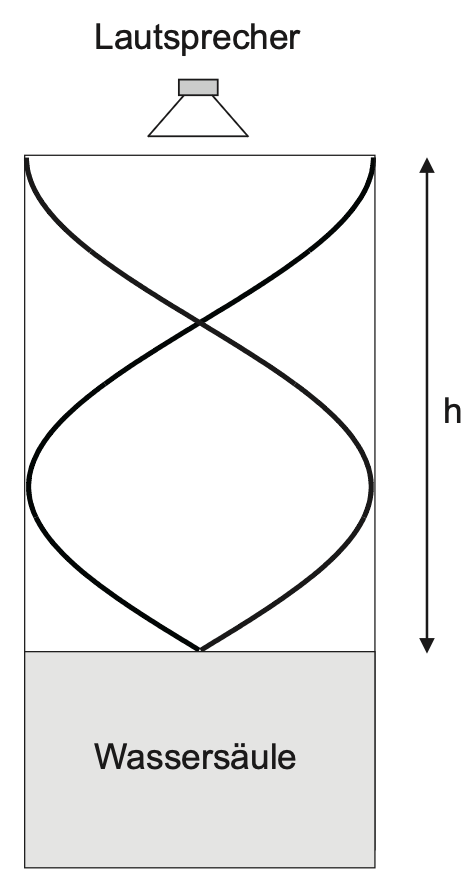
\includegraphics[width=0.2\textwidth]{img/Versuchsaufbau_Skizze.png}
    \caption{Stehende Welle im Quincke'schen Rohr.}\cite{PAPskript}
    \label{fig:stehende_welle}
\end{figure}

Für die Abstände gilt:
\begin{equation}
    \Delta s = \frac{\lambda}{2}
\end{equation}

Die Schallgeschwindigkeit kann dann aus der gemessenen Wellenlänge und der bekannten Frequenz des Lautsprechers berechnet werden.

Für die absolute Höhe h der Resonanzmaxima gilt:
\begin{equation}
    h = \frac{\left(2n + 1\right)}{4} \lambda = \frac{\left(2n + 1\right)}{4} \frac{c}{f}
\end{equation}
 
Die Schallgeschwindigkeit kann auch über eine Laufzeitmessung bestimmt werden. Hierbei wird die Phasenverschiebung zwischen dem Sendesignal eines Sinusgenerators und dem von einem verschiebbaren Mikrofon empfangenen Signal gemessen. Durch die Untersuchung der Weglängenänderung zwischen Mikrofon und Lautsprecher, bei der sich die Phase auf dem Oszilloskop um genau eine Wellenlänge (bzw. eine Periode) verschiebt, kann die Ausbreitungsgeschwindigkeit des Schalls ermittelt werden.

\begin{figure}
    \centering
    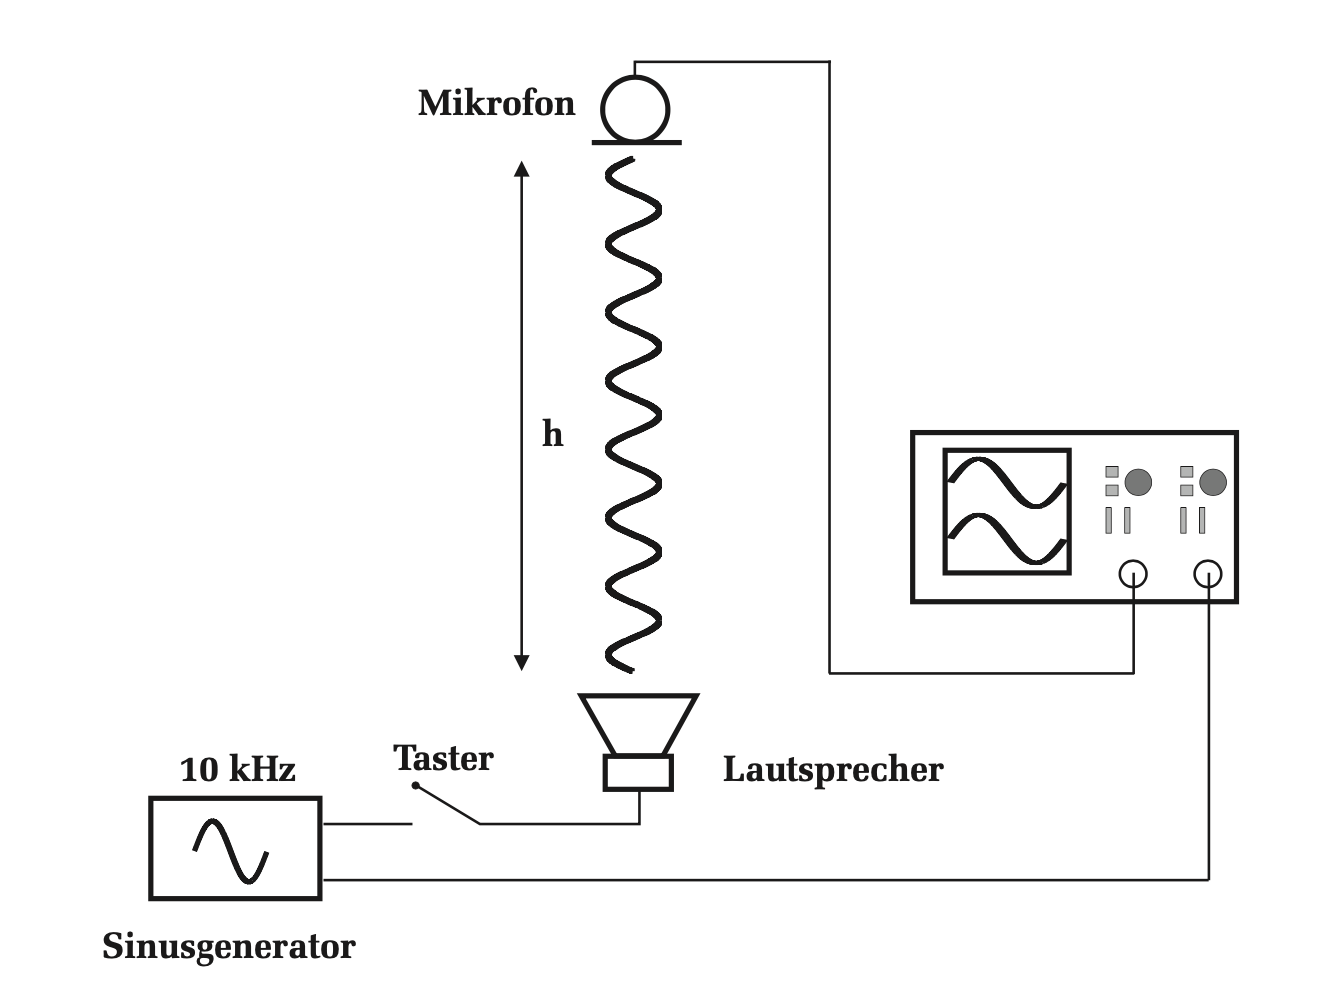
\includegraphics[width=0.5\textwidth]{img/Versuchsaufbau_Laufzeitmessung.png}
    \caption{Laufzeitmessung der Schallgeschwindigkeit.}\cite{PAPskript}
    \label{fig:laufzeitmessung}
\end{figure}

Um aus dieser Formel die Schallgeschwindigkeit zu bestimmen, wird die Phasenverschiebung $\Delta \phi$ zwischen dem Sendesignal und dem empfangenen Signal gemessen. Die Schallgeschwindigkeit kann dann aus der bekannten Frequenz $f$ und der gemessenen Phasenverschiebung berechnet werden.

\begin{equation}
    c = \frac{2\pi f \Delta x}{\Delta \phi}
\end{equation}


\subsection{Literaturwerte}
Der Literaturwert für die Schallgeschwindigkeit in Luft bei $0^{\circ}\text{C}$ beträgt:

\begin{equation}
    c_{\text{Luft,0°C}} = 331.4\,\frac{\text{m}}{\text{s}}
\end{equation}

 Bei unseren Messungen wurde die Temperatur der Luft auf $T = 25.0^{\circ}\text{C}$ gemessen, was zu einer theoretischen Schallgeschwindigkeit von:
\begin{equation}
    c_{\text{Luft,25°C}} = 346.1\,\frac{\text{m}}{\text{s}}
\end{equation}


\section{Messprotokoll}

\subsection{Versuchsaufbau und Aufgaben}
Aufgaben
\begin{itemize}
    \item Aufgabe 1: Bestimmung der Schallgeschwindigkeit in Luft und $CO_2$ mittels stehender Wellen im Quincke'schen Rohr. Dafür wurden mit einem Voltmeter die Resonanzmaxima der Schallwelle ermittelt, während die Länge der Luftsäule durch Heben des Wasserspiegels variiert wurde.
    \item Aufgabe 2: Bestimmung der Schallgeschwindigkeit in Luft durch Laufzeitmessung einer fortschreitenden Schallwelle. Hierbei wurde die Phasenverschiebung zwischen dem Sendesignal eines Sinusgenerators und dem von einem verschiebbaren Mikrofon empfangenen Signal mit einem Zweikanal-Oszilloskop gemessen. 
\end{itemize}



\pdfabbildung{Messaufbau Foto}{fig:pdf-1}
\pdfabbildung{gemessenes Signal(A2)}{fig:pdf-2}
\pdfabbildung{Lissajous-Analyse}{fig:pdf-3}
\pdftabelle{Messung mit Steigrohr}{tab:pdf-1}
\pdftabelle{Werte Laufzeitmessung}{tab:pdf-2}
\pdftabelle{Werte Laufzeitmessung - unterschiedliche Frequenzen}{tab:pdf-3}

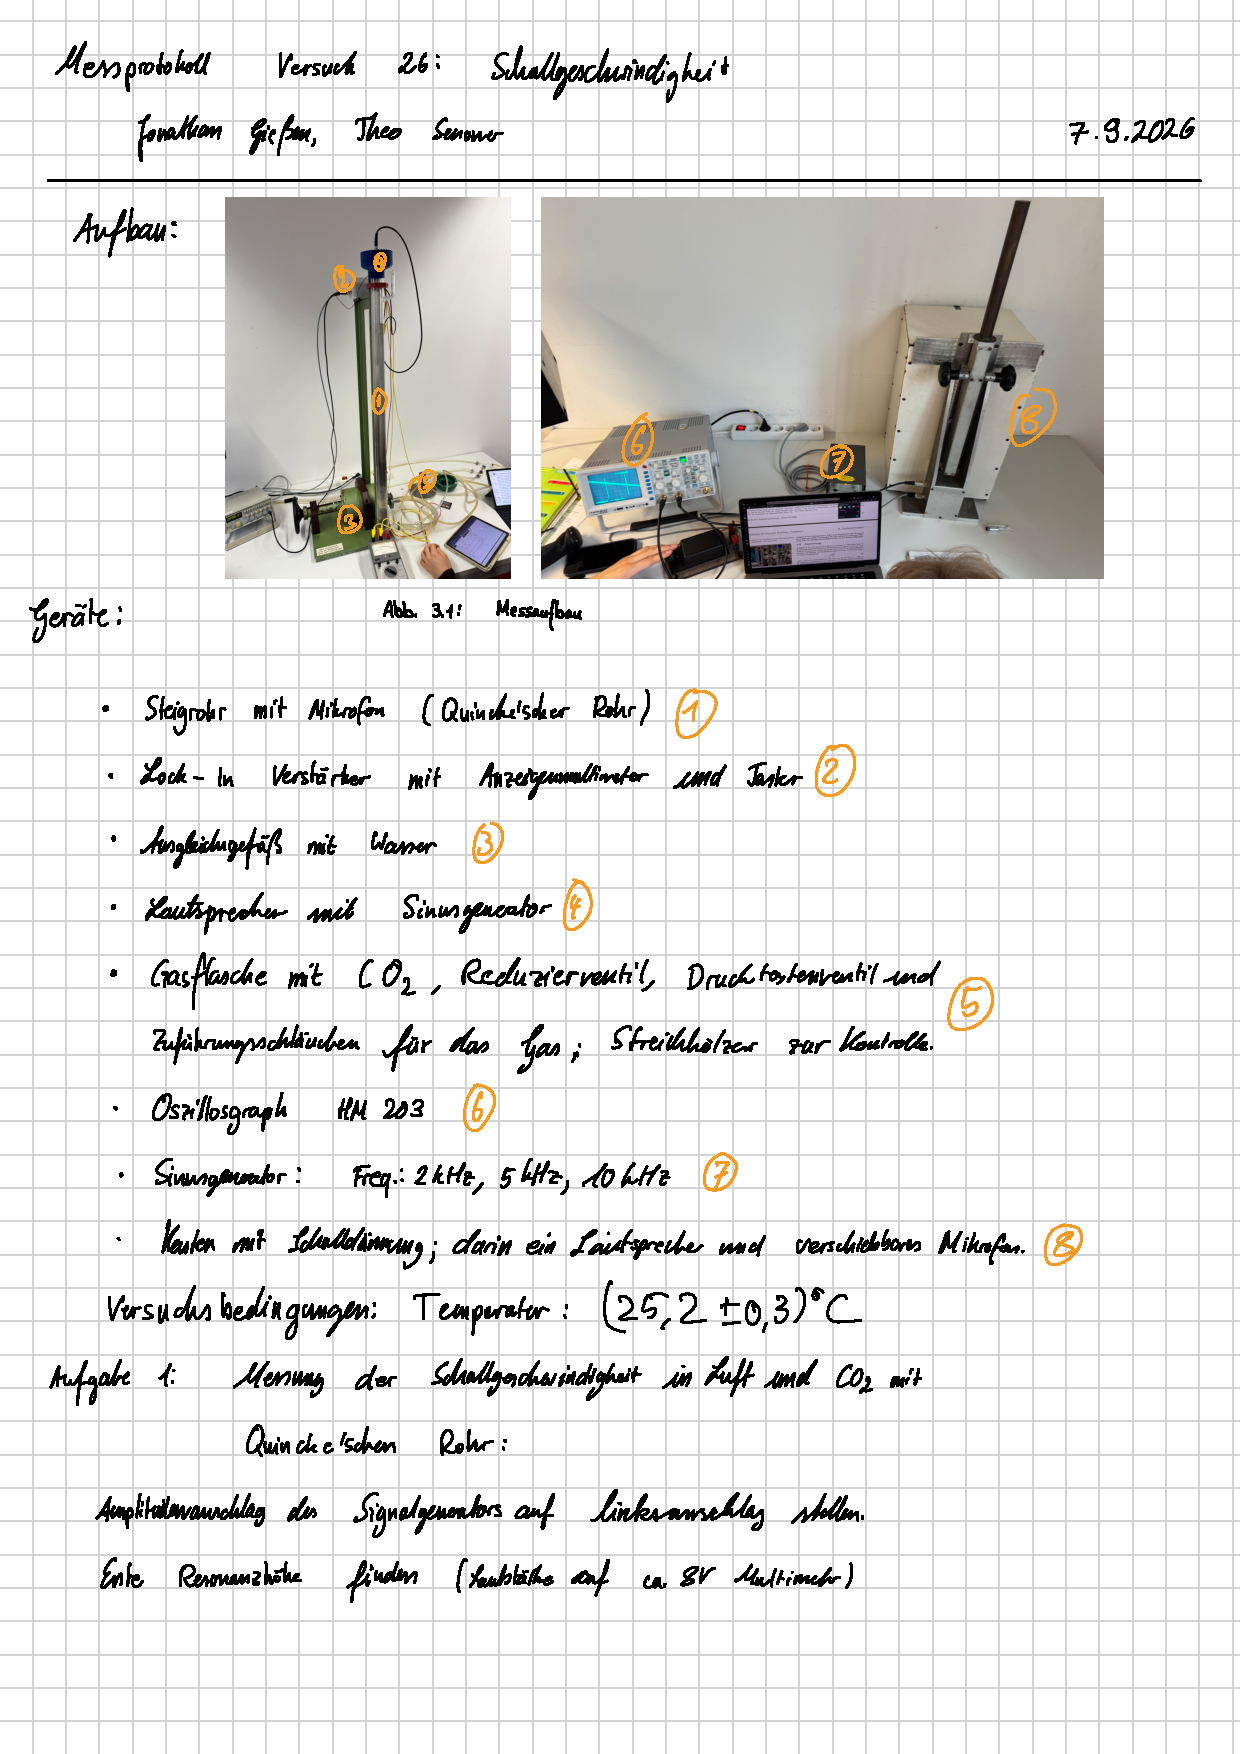
\includepdf[
    pages=-,
    width=\textwidth,
    height=\textheight,
    keepaspectratio,
    pagecommand={\thispagestyle{scrheadings}}
]{../Messprotokoll 26.pdf}

\section{Auswertung}
\subsection{Aufgabe 1: Bestimmung mithilfe des Quincke'schen Rohrs}
Aus den gemessenen Hohendifferenzen der Luftsäule im Quinschen Rohr im
Resonanzfall (Mittelwert bilden) ist die Schallgeschwindigkeit in Luft bzw. Koh-
lendioxid zu bestimmen. Nutzen Sie für die Berechnung nur die Höhendifferenzen
zwischen zwei Maxima.\cite{PAPskript}

Aus Tabelle \ref{tab:pdf-1} lassen sich die Höhendifferenzen $\Delta h$ zwischen den Resonanzmaxima für Luft und $CO_2$ ablesen. Die Wellenlänge $\lambda$ kann aus der Höhendifferenz berechnet werden, da diese der halben Wellenlänge entspricht:
\begin{equation}
    \lambda = 2 \cdot \Delta h\label{eq:wellenlaenge}
\end{equation}

Mithilfe des Angehängten Python-Skripts können die Mittelwerte der Höhendifferenzen und deren Standardabweichungen berechnet werden. 
Der Kombinierte Fehler berechnet sich durch 
\begin{equation}
    \Delta h = \sqrt{\sigma_{Werte}^2 + \Delta h_\text{mess}^2}
\end{equation}
Die Ergebnisse betragen:

\begin{table}[H]
    \centering
    \caption{Ergebisse der Wellenlängen für Luft und $CO_2$.}
    \begin{tabular}{lcc}
        \toprule
        \textbf{Substanz} & \textbf{Mittelwert} & \textbf{Wellenlänge} $\lambda$\\
        \midrule
        Luft & $\left(\Delta h_\text{Luft} = 8.65\pm 0.26\right) \text{cm} $ & $\left(17.3 \pm 0.6\right) \text{cm}$ \\
        $CO_2$ & $\left(\Delta h_\text{$CO_2$} = 6.8\pm 0.42\footnotemark\right) \text{cm} $ & $\left(14.0\pm 0.9\right)\text{cm}$ \\
        \bottomrule
    \end{tabular}
\end{table}
\footnotetext{Hier wurde die signikante Stelle missachtet, weil der Fehler dann durch Gleichung \ref{eq:wellenlaenge} zu groß wird.}


Aus den Wellenlänge und der Frequenz $\nu = (2.0050\pm 0.0020) \text{kHz}$ kann nun nach Gleichung \ref{eq:Wellenzusammenhang} die Schallgeschwindigkeit berechnet werden.

\medskip
Der Fehler berechnet sich nach der Gauß'schen Fehlerfortpflanzung:
\begin{equation}
    \Delta c = \sqrt{\left(\frac{\partial c}{\partial \lambda} \Delta \lambda\right)^2 + \left(\frac{\partial c}{\partial \nu} \Delta \nu\right)^2} = \sqrt{\left(\nu \cdot \Delta \lambda\right)^2 + \left(\lambda \cdot \Delta \nu\right)^2}
\end{equation}

Die Ergebnisse betragen:
\begin{equation}
    c_\text{Luft} = \lambda_\text{Luft} \cdot \nu = \left(347\pm 12\right) \frac{\text{m}}{\text{s}}
\end{equation}
\begin{equation}
    c_\text{$CO_2$} = \left(281\pm 18\right) \frac{\text{m}}{\text{s}}
\end{equation}

Rechnung auf Normalbedingungen ($0^{\circ}\text{C}$) mit der Formel:
\begin{equation}
    c_0 = c \cdot \sqrt{\frac{T_0}{T}}
\end{equation}

Es ergibt sich:
\begin{equation}
    c_\text{Luft,0°C} = \left(331\pm 11\right) \frac{\text{m}}{\text{s}}
\end{equation}
\begin{equation}
    c_\text{$CO_2$,0°C} = \left(268\pm 17\right) \frac{\text{m}}{\text{s}}
\end{equation}




Zur Abschätzung der relativen systematischen Messunsicherheit $\frac{\Delta q}{q}$ wird die Gauß'sche Fehlerfortpflanzung auf die Bestimmungsgleichung der Ladung angewendet:
\begin{equation}
    q = (v_f + v_s) \cdot \frac{6\pi d}{U} \sqrt{\frac{9 v_f \eta^3}{2\rho g}}
    \label{eq:q_exakt}
\end{equation}

Vergleich mit dem Literaturwert:

\begin{equation}
    c_\text{Luft,0°C} = 331.4\,\frac{\text{m}}{\text{s}}, \quad c_\text{$CO_2$,0°C} = 259.8\,\frac{\text{m}}{\text{s}}
\end{equation}

Die Unsicherheit und relative Abweichung der Messwerte von den Literaturwerten beträgt:
\begin{equation}
    \Delta c_\text{Luft,0°C} = 11\,\frac{\text{m}}{\text{s}}, \quad \Delta c_\text{$CO_2$,0°C} = 17\,\frac{\text{m}}{\text{s}}
\end{equation}
\begin{equation}
    \text{Abweichung}_\text{Luft} = \frac{|c_\text{Luft,0°C} - c_\text{Luft,0°C,lit}|}{c_\text{Luft,0°C,lit}} \approx 0.12\,\%
\end{equation}
\begin{equation}
    \text{Abweichung}_\text{$CO_2$} = \frac{|c_\text{$CO_2$,0°C} - c_\text{$CO_2$,0°C,lit}|}{c_\text{$CO_2$,0°C,lit}} \approx 3.2\,\%
\end{equation}

Das entspricht einem \sigma-Bereich von:
\begin{equation}
    \sigma_\text{Luft} = \frac{|c_\text{Luft,0°C} - c_\text{Luft,0°C,lit}|}{\Delta c_\text{Luft,0°C}} \approx 0.11 \Rightarrow 0.11\sigma
\end{equation}
\begin{equation}
    \sigma_\text{$CO_2$} = \frac{|c_\text{$CO_2$,0°C} - c_\text{$CO_2$,0°C,lit}|}{\Delta c_\text{$CO_2$,0°C}} \approx 0.94 \Rightarrow 0.94\sigma
\end{equation} 

\begin{resultbox}[Ergebnisse der Schallgeschwindigkeitsmessung]
    \begin{itemize}
        \item Schallgeschwindigkeit in Luft bei $0^{\circ}\text{C}$: $c_\text{Luft,0°C} = (331\pm 11)\,\frac{\text{m}}{\text{s}}$
        \item Schallgeschwindigkeit in $CO_2$ bei $0^{\circ}\text{C}$: $c_\text{$CO_2$,0°C} = (268\pm 17)\,\frac{\text{m}}{\text{s}}$
        \item Abweichung von Literaturwerten:
        \begin{itemize}
            \item Luft: $\approx 0.12\,\%$ ($\approx 0.11\sigma$)
            \item $CO_2$: $\approx 3.2\,\%$ ($\approx 0.94\sigma$)
        \end{itemize}
    \end{itemize}
    Das zeigt dass die bestimmten Werte innerhalb der Unsicherheiten mit den Literaturwerten übereinstimmen.
\end{resultbox}



\subsection{Abschätzung des statistischen Fehlers aus der Mehrfachmessung}


\subsection{Vergleich des Ergebnisses mit dem Literaturwert}



\section{Diskussion}
\subsection{Interpretation der Signifikanzen}

\medskip
\noindent

\subsection{Fazit}
Zum Ende lässt sich festhalten, dass die experimentelle Bestimmung der Elementarladung mit dem Millikan-Versuch 
erfolgreich durchgeführt wurde. Die Ergebnisse stimmen innerhalb der Unsicherheiten mit dem Literaturwert überein, und die Analyse der Fehlerquellen liefert wertvolle 
Einblicke in die Genauigkeit und Präzision des Versuchsaufbaus.

\clearpage

\listoffigures


\listoftables

\begin{thebibliography}{5}
    \bibitem{PAPskript} Dr. J.Wagner, \emph{Physikalisches Anfängerpraktikum}, Stand 11/2024
    \bibitem{ilberg1988physikalisches} W. Ilberg, M. Krötzsch, \emph{Physikalisches Praktikum für Anfänger}, BSB B. G. Teubner Verlagsgesellschaft, Leipzig (1985).
    \bibitem{demtroeder2017} W. Demtröder, \emph{Experimentalphysik 1: Mechanik und Wärme}, Springer Verlag, Berlin (2017).
\end{thebibliography}



\end{document}